\subsection{Material selection}
	
	The main structural components are beams that, for client requirements, should be standard and so for this reason T slot extruded aluminium profiles (figure \ref{fig:tslot:crosssectionexample}) are chosen after the following considerations:
	\begin{itemize}
		\item better volume-to-price ratio and lower density (respect to inox steels), so reducing costs associated to the spare parts and shipping;
		\item availability in the market: there are a lot of vendors that provide profiles with various geometrical dimensions, different aluminium alloy and surface finishes. This spare parts can be easily accessed by every private costumer;
		\item for T slot extruded profiles lots of auxiliary components (such supporting brackets, fasteners, hinges...)  are provided from the same profiles manufacturers, reducing the need of custom made part and so decreasing the overall costs.
	\end{itemize}

	This elements can be also purchased with an anodized finish that allows to improve the corrosion resistance, increasing so the expected life time of the product in uncontrolled outdoor environment.
	
	\begin{SCfigure}[1.5][bh]
		\centering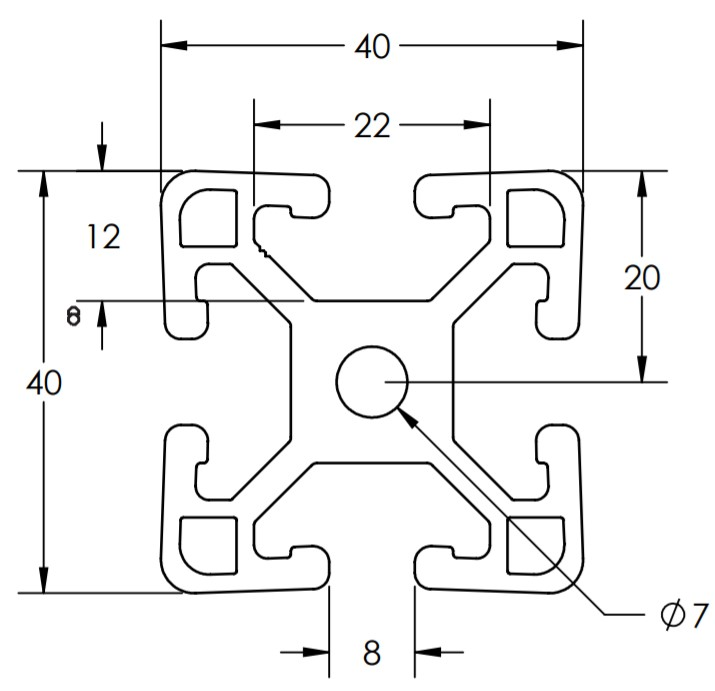
\includegraphics[width=5cm]{tslot-profile-example}
		\caption{technical drawing of a T-slot profile's cross-section. The particular sketch represent the model \texttt{TS40-40LM} by Tslots \cite{tslot-ds}.}
		\label{fig:tslot:crosssectionexample}
	\end{SCfigure}
	
	\paragraph{Mechanical properties} For the design part the following mechanical properties are considered: ultimate tensile strength $\sigma_{uts} = 260 MPa$, yielding strength $\sigma_{ys} = 240 MPa$, Young's module $E = 70 GPa$, Poisson's ratio $\nu = 0.32$; this values are chosen according to table \ref{tab:beammaterial} (page \pageref{tab:beammaterial}) as  they represent a lower bound (implying higher safety in calculations) for the aluminium material used for the T-Slot sections.
	
	
	
		
	
	
	
	
	
	
	
	
	
	
	
	
	